\chapter{Event Reconstruction}
\label{chapter:reconstruction}

The Compact Muon Solenoid, comprised of millions of individual detector channels, cannot by itself give us information about what particles have traveled through its volume; it can only offer a readout of hits in the muon and tracking detectors, energy deposits in the calorimeters, and other basic electronic signals.  The trajectories and identities of the particles which induced that detector response must be inferred through reconstruction algorithms which draw on the raw detector data to build a more coherent picture of a collision event.  The success of this analysis thus rests both on the successful functioning of the detector hardware and on the logic which builds electrons, muons, and \MET from the hardware output.  An initial view of such reconstructed output can be seen in Fig.~\ref{fig:visualization} which visualizes the content of a recorded $WZ$ event.

\begin{figure*}
  \centering
  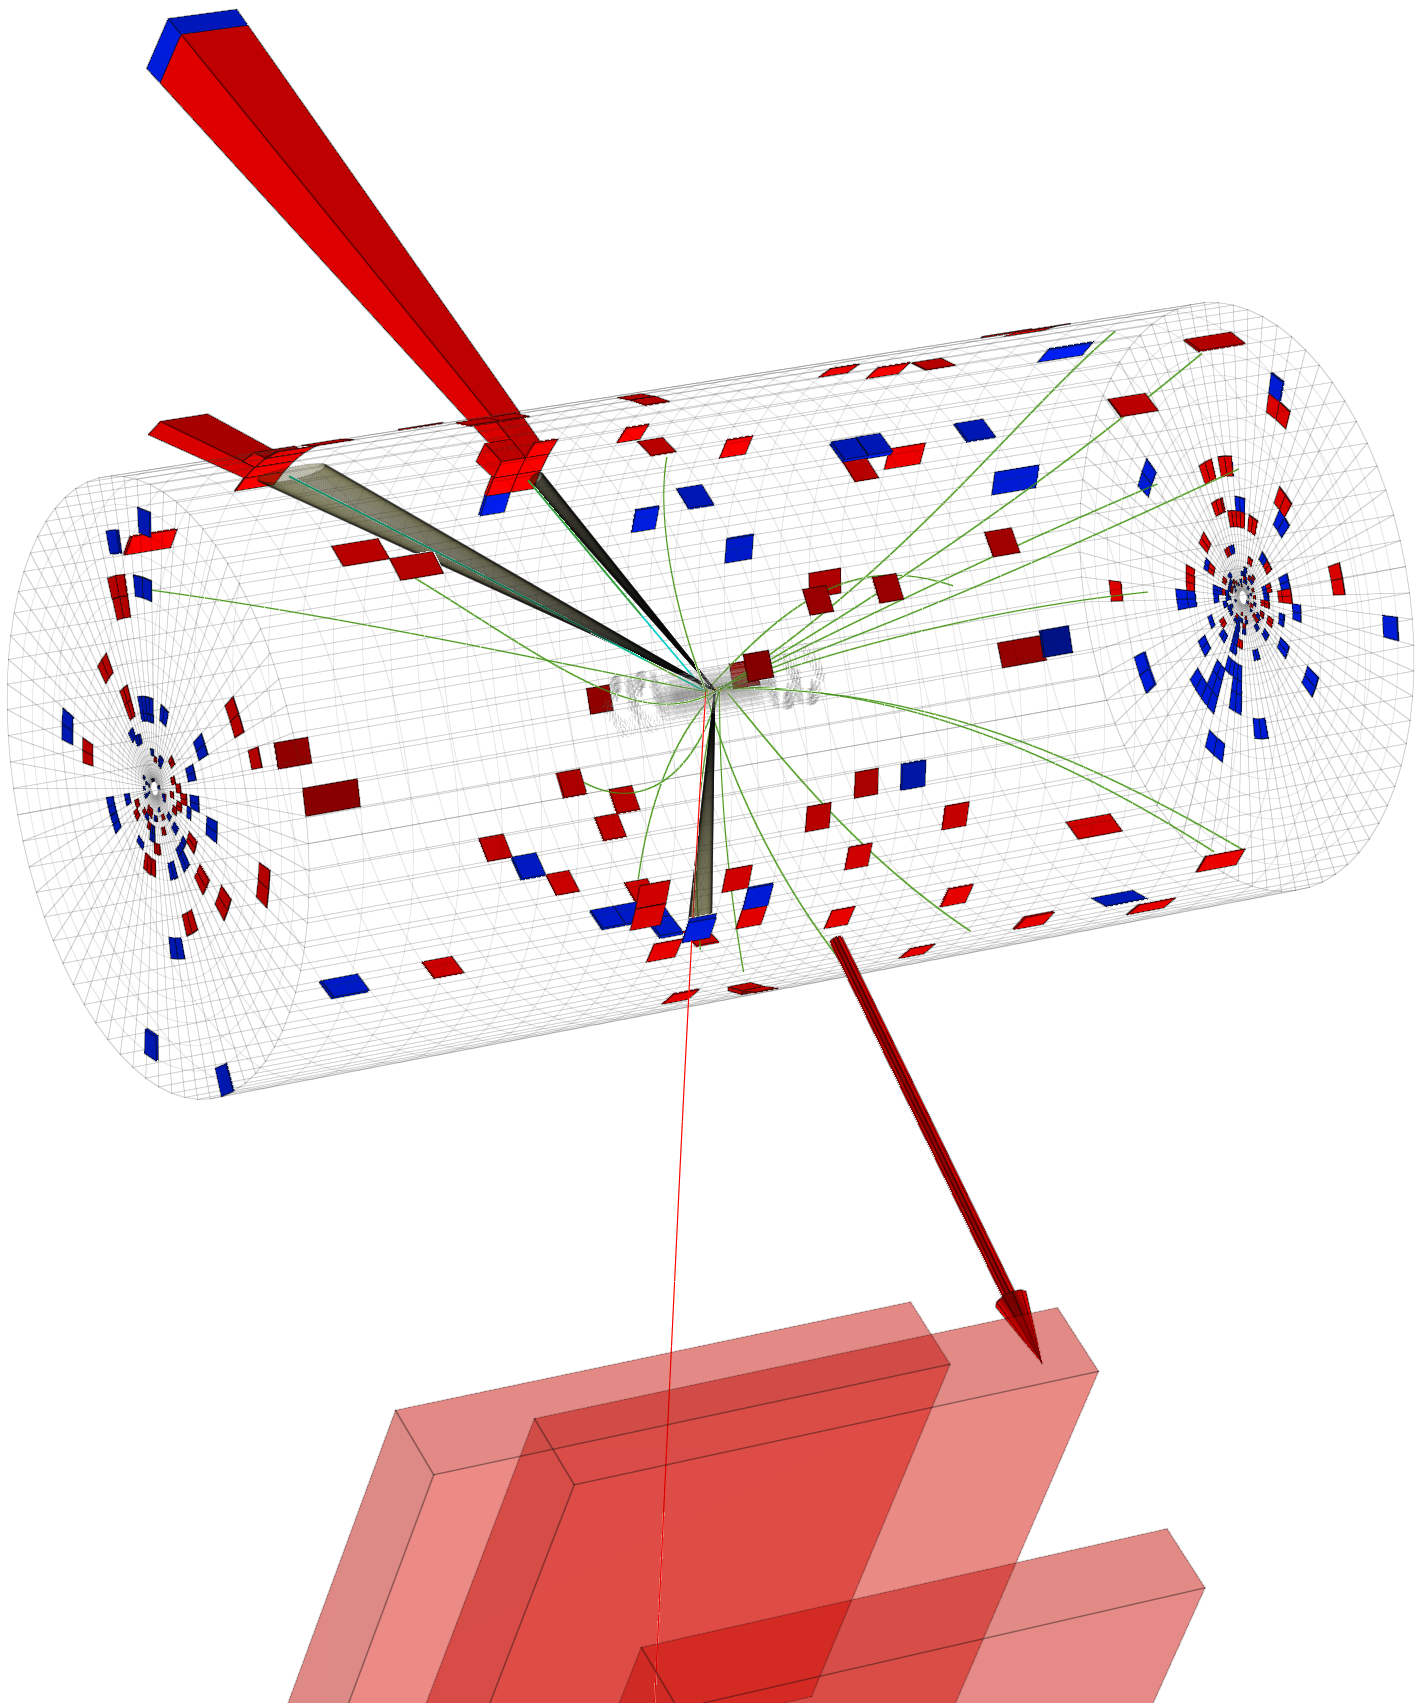
\includegraphics[width=\plotwidth]{figures/displays/167103.79.73561307.png}
  \caption[Visualization of a $WZ$ event in CMS]{Visualization of a $WZ$ event in CMS (Run 167103, Event 73561307, recorded Friday, 17 June 2011).  The wireframe shows the volume of the inner tracker, with generic reconstructed tracks drawn in green.  The heights of red and blue columns resting on the wireframe surface indicate the magnitudes of energy deposits in the \ecal and \hcal respectively.  The $Z$ boson has decayed into two electrons, emerging from the far side of the tracker; they appear as light blue tracks accompanied by large \ecal deposits.  The $W$ boson has decayed into a muon and a neutrino (indicated by the large \MET arrow) in the foreground; the muon track is shown in red, extending outward to the muon chambers (shown as translucent red blocks).}
  \label{fig:visualization}
\end{figure*}


\section{Electron Reconstruction}

\begin{figure*}
  \centering
  \subbottom[An electron passing through the tracker, then depositing energy in the \ecal{} crystals.  Note the distinct energy cluster due to a \brem{} photon.]{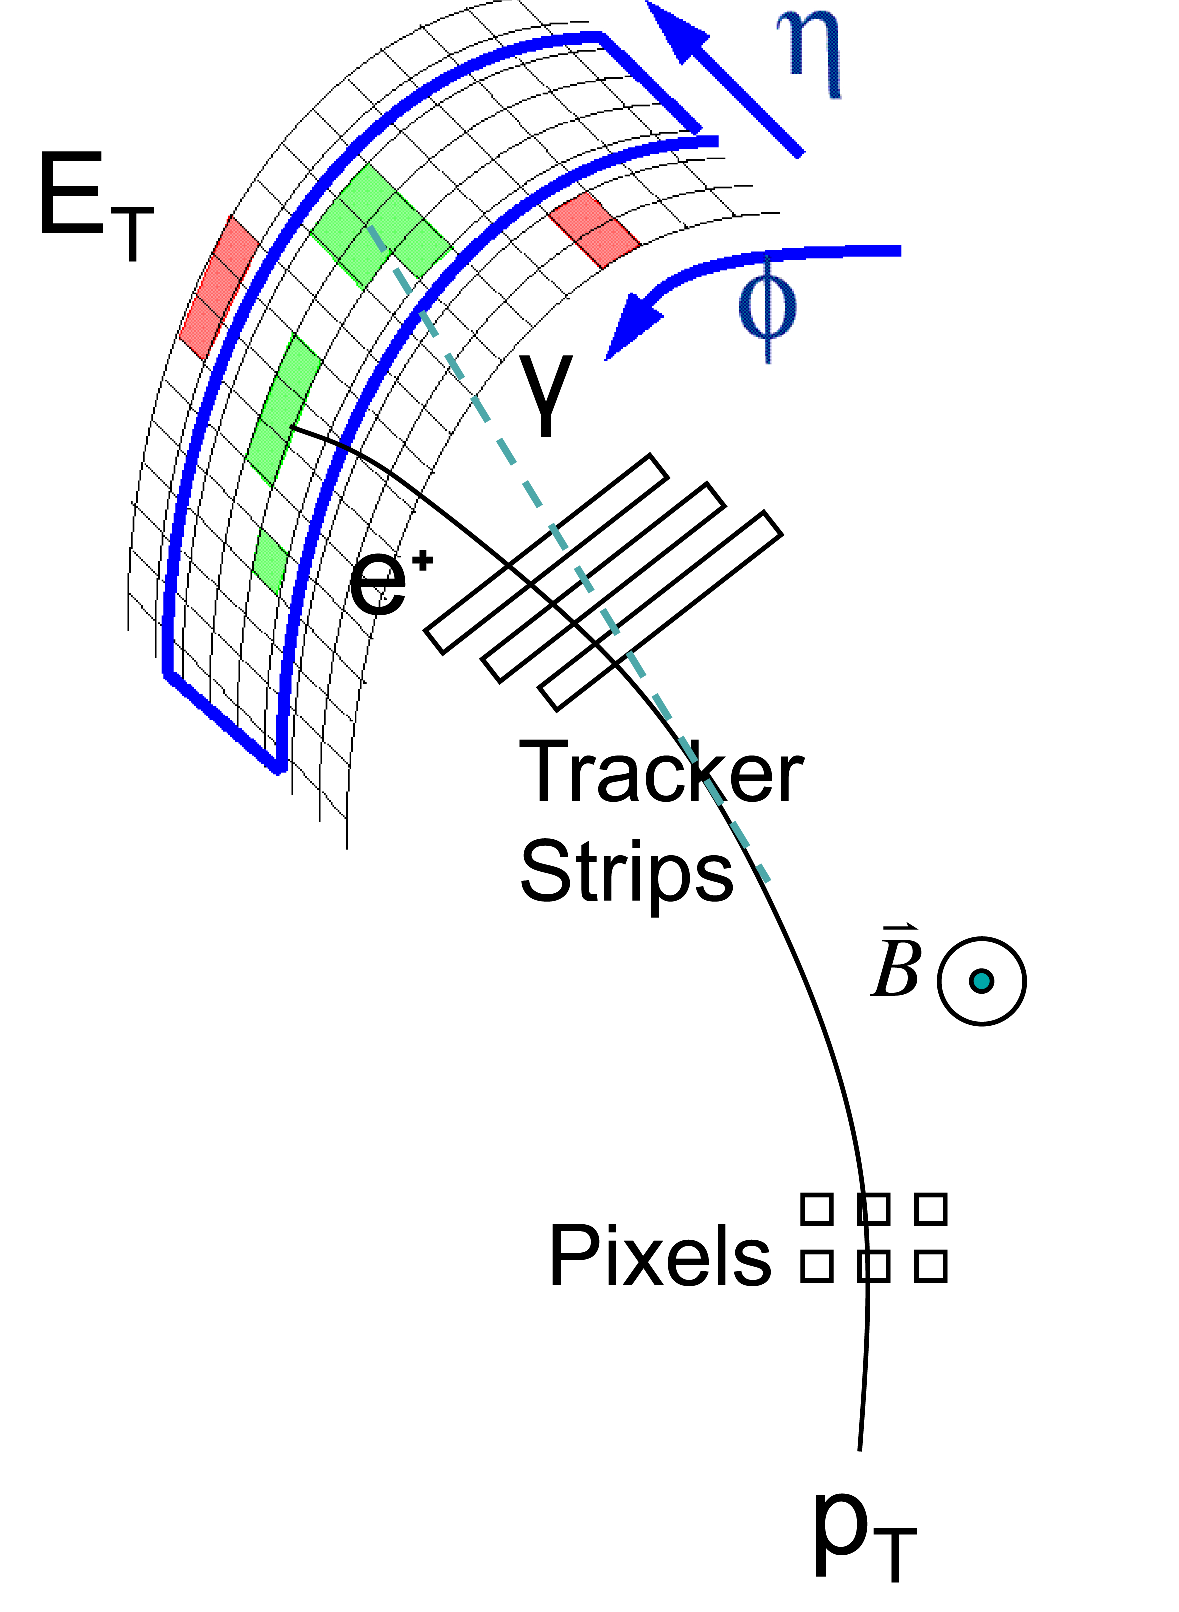
\includegraphics[width=0.47\textwidth]{figures/cms-electron-reco}\label{fig:cms-electron-reco}}
  \hfill
  \subbottom[Transverse event display showing the coincidence of a high-momentum track and a significant deposit of energy in the \ecal{} characteristic of an electron.]{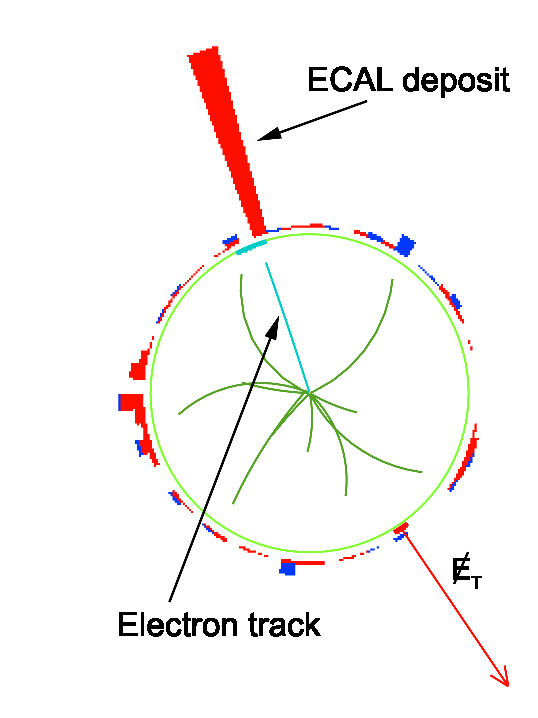
\includegraphics[width=0.47\textwidth]{figures/cms-electron-display}\label{fig:cms-electron-display}}
  \caption{Two diagrams showing the response of the CMS detector to a high-energy electron.}
  \label{fig:cms-electron-diagrams}
\end{figure*}

The basic signature for an electron in CMS is an ECAL energy deposit matched to a track in the inner tracker, which the CMS reconstruction software identifies via two complementary algorithms~\cite{CMS-PAS-EGM-10-004}.  The ``tracker-driven'' algorithm is optimized for low-\pt electrons and those inside jets, starting from a collection of tracks and looking for corresponding clusters of energy in the \ecal.  The ``\ecal-driven'' algorithm, however, is more relevant to this analysis since it is optimized for isolated electrons in the \pt range under consideration (\pt > 10).  As implied by its name, this technique starts in the \ecal, grouping together associated clusters of energy into ``superclusters'' which are narrow in $\eta$ but may have a significant spread in $\phi$, characteristic of an electron bending in the magnetic field and radiating as it passes through the tracker material.  Once these superclusters are identified, they are matched not with reconstructed tracks, but rather with pairs or triplets of hits in the innermost layers of the tracker.  These hits are used as seeds for a special electron tracking algorithm which takes into account a model of the typical electron energy loss when moving through the tracker.

At this reconstruction stage, some loose quality requirements are imposed to remove faulty candidates while maintaining an efficiency above 99\% for isolated electrons.  The ratio of energy deposited in the \hcal vs. the \ecal in the supercluster region must fall below 0.15 as significant deposits in the \hcal would indicate hadronic activity from a jet.  In addition, the displacement between the supercluster centroid and its associated track must fall within the bounds $\Delta\eta < 0.02$ and $\Delta\phi < 0.15$.  In general, the requirements imposed at the analysis level are more strict and supersede these reconstruction-level criteria.  Additionally, these requirements are loose enough that the objects classified as reconstructed electron candidates can be used to study other physics objects being misidentified as electrons.  The electron four-momentum and point of origin are assigned based on the track parameters at the distance of closest approach to the nominal beam spot, with the energy determined from a combination of tracker and \ecal information.


\section{Muon Reconstruction}
Muon reconstruction in CMS starts from local pattern recognition in each of the muon subsystems, followed by ``stand-alone'' and ``global'' reconstruction algorithms~\cite{CMS-MuonReco}.  The stand-alone reconstruction phase integrates information throughout the muon subsystems, linking together track segments from the individual chambers and fitting them into stand-alone muon tracks.  This algorithm looks for seeds in the innermost chambers, first building tracks outward using a Kalman-fitter technique~\cite{Fruhwirth1987444}, then refitting inward to define track parameters at the innermost muon station.  These stand-alone muons are then compared to independently-reconstructed tracks from the inner tracker by propagating those tracks to the inside surface of the muon detector.  Compatibility in terms of momentum, position, and direction are considered in matching stand-alone muons to tracker tracks and the hits from matched pairs are used as input for a new, global fit.  The resulting collection of global muon tracks may contain ambiguities and poor matches, so arbitration and quality algorithms are applied to choose at most one final global track to associate with each stand-alone muon.

While the inner tracker can in general provide a much higher momentum resolution than the muon system due to its high granularity and the greater multiplicity of hits available for the track fit, the combination of these two systems becomes important for muons with momentum above \simomentum{100}.  At high energies, the reduced bending of the muon tracks limits the resolution of the inner tracking algorithms.  In these cases, just a few hits at the large radius of the muon system can significantly improve the curvature measurement, constraining the fit and providing a better momentum resolution.  A high-quality muon is expected to have at least one hit within the muon chambers and at least one within the inner pixel tracker, with a greater multiplicity of hits generally correlated with a better-reconstructed track.  The quality of the fit is estimated through a normalized $\chi^2$ determination.  Prompt muons can be distinguished from secondary muons produced in hadronic decays through measurement of the impact parameter of the track with respect to the primary vertex.

As an alterative to stand-alone and global muons, CMS employs an algorithm for identifying ``tracker muons'' which consist of tracks in the inner tracker matched to individual muon segments.  In this scenario, all tracks with $\pt > \simomentum{0.5}$ and total momentum $p > \simomentum{2.5}$ act as seeds and are considered as muon candidates if they can be matched to at least one muon segment.  While this approach can be particularly useful for low-\pt studies where the global reconstruction algorithm degrades, it maintains a high efficiency over the entire muon \pt range.  For this analysis, we use this tracker-driven algorithm as a cross-check for muon quality; all global muons considered in the analysis must also be identified as tracker muons.

\section{Jet Reconstruction}
\label{sec:jet-reco}

While both electron and muon reconstruction algorithms are able to use the high granularity of the tracker as a clear guide towards deposits elsewhere in the detector, jets are partially composed of neutral particles which do not leave tracks, necessitating a significant reliance on the calorimeters.  As a result, a direct search for jets introduces ambiguity which limits the effectiveness of reconstruction algorithms.  This difficulty motivates the CMS particle flow algorithm~\cite{ParticleFlow} which seeks to provide a more nuanced view of an event by reconstructing physics objects in sequence, removing tracker hits and energy deposits from consideration once they are assigned to a particular object.  In this approach, muons are reconstructed first, accounting for all segments in the muon chambers while removing related tracks in the tracker and energy deposits in the calorimeter before moving on to electrons and jets.  The input to the jet reconstruction algorithm, then, is a collection of energy deposits which have a high likelihood of belonging to a jet, allowing for a more efficient reconstruction.

Within the context of particle flow, jets are created by means of the ``anti-$k_\text{T}$'' clustering algorithm~\cite{antikt} which looks for a high-momentum particle as a seed, then adds nearby particles to the jet with weights corresponding to their momenta.  This algorithm is both ``infrared safe'' in the sense that it is not affected by the presence of the infinitely soft particles which result from QCD divergences and also ``collinear safe'' in the sense that it automatically recombines collinear partons~\cite{Ellis:1993tq}.  These two qualities are essential to allow meaningful comparisons between reconstructed jets and theoretical calculations to arbitrary order.  

\section{Pileup}
\label{sec:pileup}

The intense luminosity provided by the LHC creates an environment where each bunch crossing can lead to dozens of individual $pp$ collisions.  While the high resolution of the tracker allows association of charged particles to distinct vertices, the same technique cannot be used for neutral particles which leave no signature in the tracker.  For jet measurements in particular, the heavy reliance on calorimeters limits the ability to distinguish vertices.  In most events of interest, there is only one hard scattering interaction; the various other proton collisions, known as \emph{pileup}, are typically soft, leading to significant jet activity, particularly in the forward regions of the detector.  The number of pileup interactions in a given bunch crossing has a significant effect on our resolution for jet energy measurements, motivating an event-by-event treatment to correct for these effects.

One of the major treatments for this type of pileup correction at CMS is the \textsc{fastjet} algorithm~\cite{Cacciari:2007fd,Cacciari:2008gn} which estimates an energy contribution due to pileup for each reconstructed jet which can then be subtracted from the jet's energy to yield a result which more closely represents the energy of the initiating parton.  The algorithm proceeds by assigning an abstract ``area'' $A$ to each jet which is essentially a measurement of its susceptibility to pileup contamination while measuring the overall level of diffuse noise $\rho$ in the event as the median value of $\pt/A$ taken over all jets.  In the analysis given here, the \textsc{fastjet} algorithm will be important for applying pileup corrections to the isolation sums considered for identification of leptons (see Secs.~\ref{sec:electron-selection} and~\ref{sec:muon-selection}).

\section{Missing Transverse Energy}
\label{sec:met}

Although the neutrino produced in a $W \to \ell \nu$ decay will leave no deposits within the detector, we can use the visible particles in the event and the principle of momentum conservation to infer its presence.  Although the center of momentum in a hard interaction at the LHC may carry a significant longitudinal boost with respect to the lab frame, the interacting partons should have negligible momentum transverse to the beampipe.  The vector sum of the transverse momenta of the decay products, therefore, should be very small in magnitude, and any significant imbalance would indicate the direction and momentum of a particle which escaped the detector without interacting.

Such an imbalance is traditionally known as missing transverse energy (\MET), with the measurement relying on calorimetric information.  The hermetic coverage of the CMS calorimeters lends itself well to this kind of measurement, and indeed the CMS reconstruction software defines a calorimeter-based \MET vector:
\begin{equation}
  \vecMET \equiv - \sum_{i} \vec{E}_\text{T}(i),
\end{equation}
where $i$ iterates over all energy deposits in the calorimeters and $\vec{E}_\text{T}(i)$ is the transverse projection of a vector with magnitude equal to the selected energy deposit, pointing from the interaction region toward the deposit.

This relatively simple definition of \MET, however, does not fully exercise the capabilities of the CMS detector since it ignores the various tracking systems and makes no effort to match the energy deposits to any particle hypothesis which might help distinguish their origin.  As with jet reconstruction, significant resolution can be gained for \MET by taking a particle flow approach.

Within the context of particle flow, missing transverse energy can be calculated from the vector sum of the transverse momenta for all reconstructed particles:
\begin{equation}
  \vecMET \equiv - c \sum_{i} \vec{p}_\text{T}(i),
\end{equation}
where $i$ iterates over all objects identified by the particle flow algorithm.  For the present analysis, we prefer the dedicated electron and muon reconstruction algorithms over particle flow due to their comparative simplicity, but the particle flow definition of \MET has been shown to have good reliability and significantly enhanced resolution with respect to the traditional calorimetric definition and is thus suitable for use here.

